The scattering of two positively charged $\PW$ bosons with their subsequent leptonic decay with different flavours can proceed at the LHC through the partonic process:
\AK{This is only one such process...}
\MP{I added ``with different flavours'' and ``can''.}
%
\begin{equation}
\Pp\Pp\to\mu^+\nu_\mu{\rm e}^+\nu_{\rm e}\,\Pj\Pj+\mathrm{X}.
\end{equation}

This process possesses three LO contributions of different orders.
The first one is of order $\mathcal{O}{\left(\alpha^{6}\right)}$ and is referred to as the EW contribution.
In addition to typical VBS contributions, as shown on the left of Fig.~\ref{diag:LO}, it also features $s$-channel contributions.
Note that we define $s$-, $t$-, and $u$-channel contributions by looking at the process which is contained by only looking at the quark lines, {\emph i.e.}\ $s$-channel denotes all Feynman diagrams where the two initial-state partons are connected by a continuous fermion line, and $u$-channel is the contribution with crossed fermion lines, which appears for identical quarks or anti-quarks in the final state.\AK{This sentence makes no sense to me. How about: ``Note that we define $s$-, $t$-, and $u$-channel contributions by looking at the quark lines. $s$-channel denotes all the diagrams where the final state quarks are produced from the decay of a vector boson.'' Or am I missing something?}
The $s$-channel contributions will play a particular role in the study of the various contributions in Sec.~\ref{subsec:contributions}.
Some of them take the form of decay chains, for example the diagram represented in the middle of Fig.~\ref{diag:LO}, while others are tri-boson contributions (right of Fig.~\ref{diag:LO}).
When using approximations, care must be taken that only gauge-invariant subsets are considered to obtain physically meaningful results. We will discuss the commonly-used possible choices in detail in the next section.

The process can also be mediated via a gluon connecting the two quark lines while the $\PW$ bosons are radiated off the quark lines.
These contributions are of order $\mathcal{O}{\left(\alphas^{2}\alpha^{4}\right)}$ and feature different kinematical behaviours than the EW contributions.
Nonetheless they share the same final state and therefore constitute an irreducible background.

Finally, due to the specific colour structure of these two classes of amplitudes, there exist non-zero interferences if only one quark family is involved.
These are of order $\mathcal{O}{\left(\alpha_{\rm s}\alpha^{5}\right)}$ and are usually small but not negligible for realistic experimental set-ups \cite{Biedermann:2017bss}.

In experimental measurements, special VBS-cuts are designed to enhance the EW contribution over the QCD one.
These cuts are based on the fact that the two contributions have different kinematical behaviour.
The EW contribution is characterised by two jets with large rapidities as well as a large invariant mass.
The two $\PW$ bosons are mostly produced centrally.
This is in contrast to the QCD contribution which favours jets in the central region.
Therefore, the event selection usually involves rapidity-difference and invariant-mass cuts for the jets.
This will be further discussed in Sec.~\ref{subsec:contributions}.
Note that, as pointed out in Ref.~\cite{Biedermann:2017bss}, when considering full amplitudes the separation between EW and QCD production becomes meaningless.
Hence, combined measurements which are well defined theoretically should be rather performed by the experimental collaborations at the LHC.
\AK{Should we also discuss the definition of the process at NLO - ie point out that at this level one can no longer distinguish EW/QCD production?}
\MP{I added two sentences, I guess we should develop in the conclusion/recommendation part}


\begin{figure*}[t]
\begin{center}
          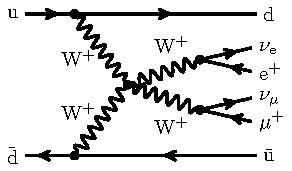
\includegraphics[width=0.30\linewidth]{feynman/LO_EW_5}
          \raisebox{.5ex}{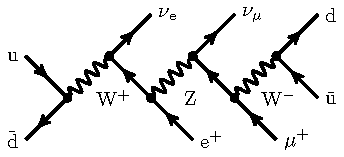
\includegraphics[width=0.35\linewidth]{feynman/LO_EW_2}}
          \raisebox{-1.8ex}{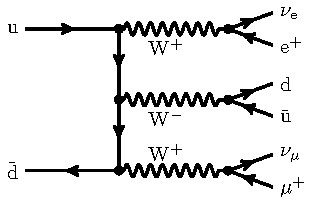
\includegraphics[width=0.32\linewidth]{feynman/LO_EW_3}}
\end{center}
        \caption{Sample tree-level diagrams that contribute to the process $\Pp\Pp\to\mu^+\nu_\mu\Pe^+\nu_{\Pe}\Pj\Pj$ at order $\mathcal{O}{\left(\alpha^{6}\right)}$.
        In addition to typical VBS contribution (left), this order also possesses $s$-channel (middle) and tri-boson contributions (right). \AK{The text here is in conflict with the main text. Reading this it looks as if s-channel and tri-boson production are two different classifications, but in the main text we say both decay chains and tri-boson production belongs to s-channel.}}
\label{diag:LO}
\end{figure*}
